%%%%%%%%%%%%%%%%%%%%%%%%%%%%%%%%%%%%%%%%%%%%%%%%%%%%%%%%%%%%%%%%%%%%
%% I, the copyright holder of this work, release this work into the
%% public domain. This applies worldwide. In some countries this may
%% not be legally possible; if so: I grant anyone the right to use
%% this work for any purpose, without any conditions, unless such
%% conditions are required by law.
%%%%%%%%%%%%%%%%%%%%%%%%%%%%%%%%%%%%%%%%%%%%%%%%%%%%%%%%%%%%%%%%%%%%

\documentclass{beamer}
\usetheme[faculty=ped]{fibeamer}
\usepackage[utf8]{inputenc}
\usepackage[
  main=english, %% By using `czech` or `slovak` as the main locale
                %% instead of `english`, you can typeset the
                %% presentation in either Czech or Slovak,
                %% respectively.
  czech, slovak %% The additional keys allow foreign texts to be
]{babel}        %% typeset as follows:
%%
%%   \begin{otherlanguage}{czech}   ... \end{otherlanguage}
%%   \begin{otherlanguage}{slovak}  ... \end{otherlanguage}
%%
%% These macros specify information about the presentation
\title{ About outlier detection, normalization and algorithm selection } %% that will be typeset on the
\subtitle{International Workshop on Econometrics and Data Analytics \\ Monash Business School} %% title page.
\author{Sevvandi Kandanaarachchi }
\institute{Monash University}
%% These additional packages are used within the document:
\usepackage{ragged2e}  % `\justifying` text
\usepackage{booktabs}  % Tables
\usepackage{tabularx}
\usepackage{tikz}   % Diagrams
\usepackage[position=top]{subfig}
%\usepackage{floatrow} 
\usetikzlibrary{calc, shapes, backgrounds}
\usepackage{amsmath, amssymb}
\usepackage{url}       % `\url`s
\usepackage{listings}  % Code listings
\newcommand{\dist}{\text{dist}}
\newcommand{\argmin}{\mathop{\text{argmin}}}
\newcommand{\nn}{\text{nn}}
\newcommand{\nnd}{\text{nnd}}
\newtheorem{proposition}[theorem]{Proposition}
\frenchspacing
\begin{document}

  \frame{\maketitle}
	
  %  \begin{frame}[noframenumbering,plain]
%	\titlepage
  %  \end{frame}

  \begin{darkframes}


    \begin{frame}[noframenumbering,plain]
    {Joint work with}
    \begin{figure}
    \captionsetup[subfigure]{labelformat=empty}
    \centering
	\subfloat[Mario A Mu\~{n}oz]{
		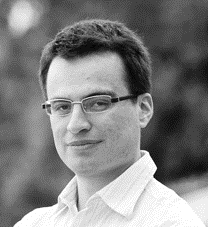
\includegraphics[scale=0.5]{Andres.png}
		%\caption{}
	}\hspace{0.5cm}%
	\subfloat[Rob Hyndman]{
		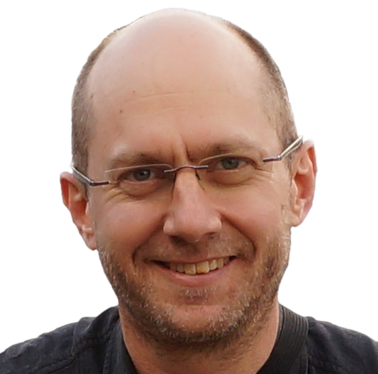
\includegraphics[scale=0.5]{Rob.png}
		%\caption{}
	}\hspace{0.5cm}%
	\subfloat[Kate Smith-Miles]{
		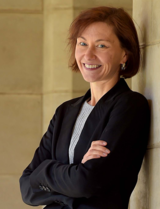
\includegraphics[scale=1.75]{Kate.png}
		\label{Kate}
		%\caption{}
	}%
  \end{figure}  
    \end{frame}

	\begin{frame}[noframenumbering,plain,label=figs1]
		\begin{figure}[b]
		\centering
		\tikzset{
			head/.style = {fill = none, label = center:\textsf{H}},
			tail/.style = {fill = none, label = center:\textsf{T}}}
		\scalebox{0.65}{\begin{tikzpicture}[
			scale = 1.5, transform shape, thick,
			every node/.style = {draw, circle, minimum size = 10mm},
			grow = down,  % alignment of characters
			level 1/.style = {sibling distance=3cm},
			level 2/.style = {sibling distance=4cm},
			level 3/.style = {sibling distance=2cm},
			level distance = 2.25cm]
			\node[shape = rectangle,
			minimum width = 6cm, minimum height = 1.5cm, font = \sffamily, rounded corners, fill={rgb:red,0;green,176;blue,80}] {About outlier detection};
	
			
			% Labels
		\end{tikzpicture}}
	\end{figure}
	
	\end{frame}

\begin{frame}[noframenumbering,plain]{Outlier detection}
\begin{itemize}
    \item It means different things to different people
    \item What is the definition of an outlier?
    \item We focus on ground truth when labelling outliers
\end{itemize}
\end{frame}

\begin{frame}[noframenumbering,plain]{Ground truth as an outlier}
    \begin{itemize}
        \item Red dot - an alien, black dots - humans
    \end{itemize}
    \begin{figure}
    \captionsetup[subfigure]{labelformat=empty}
     \centering
	\subfloat[Figure 1]{
		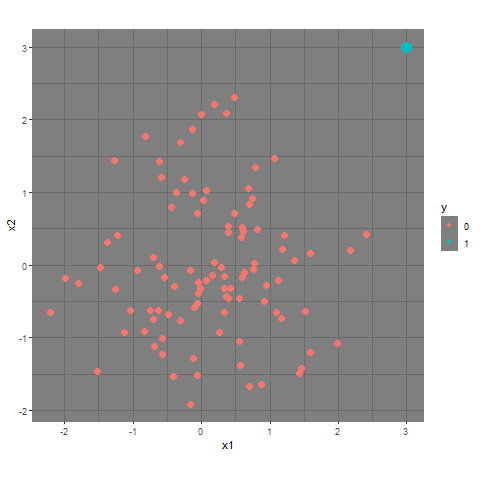
\includegraphics[width=0.48\textwidth]{example1.png}
		%\caption{}
	}%
	\subfloat[Figure 2]{
		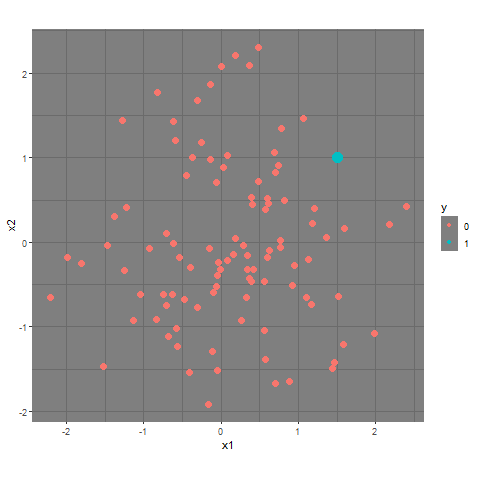
\includegraphics[width=0.48\textwidth]{example2.png}
		%\caption{}
	}
	\end{figure}
    
\end{frame}

\begin{frame}[noframenumbering,plain]{Disagreement between outlier methods}
       \begin{figure}
    \captionsetup[subfigure]{labelformat=empty}
     \centering
		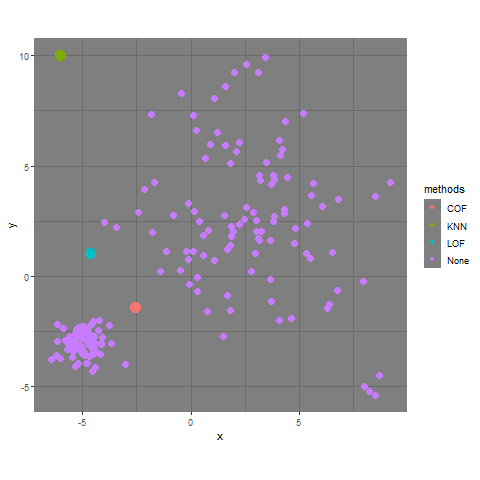
\includegraphics[width=0.8\textwidth]{example3.png}
	\end{figure}
\end{frame}

\begin{frame}[noframenumbering,plain]{Research Question 1 - Algorithm Selection}
    \centering
    {\huge What is the best outlier detection } \\ \vspace{0.5cm}
    {\huge method for my problem?}
\end{frame}	

	\begin{frame}[noframenumbering,plain]{More Questions - Normalization}
	\begin{itemize}
		\item Why normalize?
		\item Traditionally min-max normalization is used
		\item All columns are normalized to $[0, 1]$
		\item Other methods available - column by column
		\begin{itemize}
			\item Mean-SD
			\item Median-IQR
			\item Median-MAD
		\end{itemize}
		\vspace{1cm}		
		\item { \Large Why does it matter? }
		\end{itemize}
	\end{frame}

	\begin{frame}[noframenumbering,plain]{Because . . .}
	\centering
	{\Huge Performance may suffer! }
	\end{frame}

	\begin{frame}[noframenumbering,plain]{LOF - an Example}
	LOF - Local outlier factor \\
	(Breunig {\it et. al. })
	
	\begin{figure}[H]
	\centering
	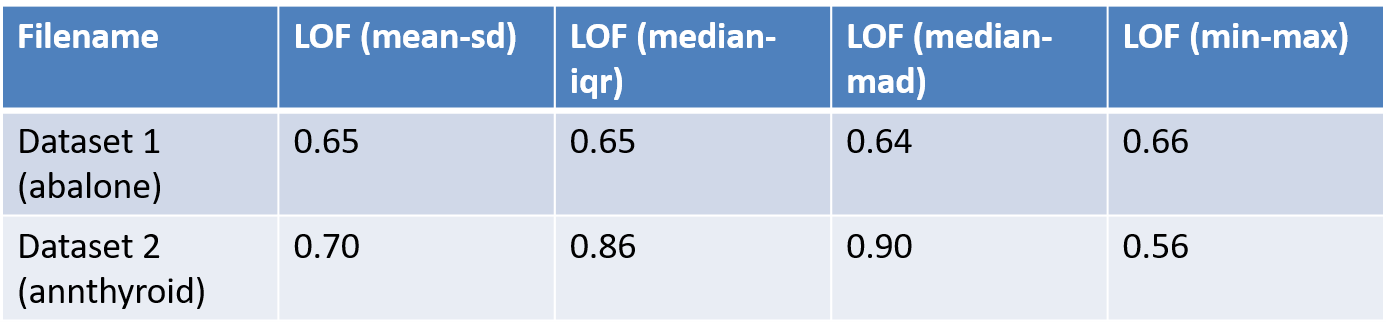
\includegraphics[scale=0.4]{LOF_Example.png}
	\end{figure}
	\end{frame}
	
	\begin{frame}[noframenumbering,plain]{Research Question 2 - Normalization}
	 \centering
	  {\huge Can we understand the effect of}\\ \vspace{0.5cm}
	  {\huge normalization on outlier detection?}
	\end{frame}
	
		\begin{frame}[noframenumbering,plain,label=figsnorm]
		\begin{figure}[b]
		\centering
		\tikzset{
			head/.style = {fill = none, label = center:\textsf{H}},
			tail/.style = {fill = none, label = center:\textsf{T}}}
		\scalebox{0.65}{\begin{tikzpicture}[
			scale = 1.5, transform shape, thick,
			every node/.style = {draw, circle, minimum size = 10mm},
			grow = down,  % alignment of characters
			level 1/.style = {sibling distance=3cm},
			level 2/.style = {sibling distance=4cm},
			level 3/.style = {sibling distance=2cm},
			level distance = 2.25cm]
			\node[shape = rectangle,
			minimum width = 6cm, minimum height = 1.5cm, font = \sffamily, rounded corners, fill={rgb:red,0;green,176;blue,80}] {About Normalization};
			

			% Labels
		\end{tikzpicture}}
	\end{figure}
	
	\end{frame}

	
	\begin{frame}[noframenumbering,plain]{WHY does normalization affect outlier detection?}
	\begin{itemize}
		\item Each axis is squashed/stretched differently
		\item Normalization changes distances
		\item Nearest neighbour structure changes
		\item Changes densities
		\vspace{1cm}
		\item {\Large Most outlier detection methods work on distances or densities}
		
	\end{itemize}
	\end{frame}

	\begin{frame}[noframenumbering,plain]{Giving some notation \ldots }
	Let  $\mathbf{x}_i \in \mathbb{R}^d$. Normalizing it we get 
	\begin{equation*}\label{eq:norm1}
	\mathbf{x}^*_i = S^{-1}\left(\mathbf{x}_i - \mu \right) \, .
	\end{equation*}
	Here $\mathbf{x}^*_i$ is the normalized observation,  \\
	$\mu$ is minimum/mean/median  \\
	$S$ is a diagonal matrix containing column-wise range/standard deviation/IQR/MAD. \\
	 Let $S = \diag(s_1, s_2, s_3, \dots, s_d)$ . %If the range, standard deviation, IQR or MAD of a certain column $k$ is zero then we assign $1$ to $s_k$, i.e.\ we leave column $k$ unchanged. This assures  $S$ is  invertible. \margincomment{Shall we remove the zero denominator part? Need to say S is invertible.}  
	
	\begin{equation*}\label{eq:norm2}
	\dist(\mathbf{x}^*_i, \mathbf{x}^*_j) = \left\lVert S^{-1}\left(\mathbf{x}_i - \mathbf{x}_j \right) \right\rVert \, ,
	\end{equation*}
	\end{frame}	

	\begin{frame}[noframenumbering,plain]{Mathematically we show \ldots  }
    \begin{itemize}
        \item Depending on the normalization scheme
        \begin{itemize}
            \item Nearest neighbours change
            \item Densities change
        \end{itemize}
        \item Normalization scheme can mask the true outliers and favour non-outliers  
    \end{itemize}
    \end{frame}

    \begin{frame}[noframenumbering,plain]{Any real data?}
        \centering
        {\huge We did a BIG experiment!}
    \end{frame}

  	\begin{frame}[noframenumbering,plain]{Our experiment with real data}
 	\begin{itemize}
 		\item 12000+ datasets
 		\begin{itemize}
 			\item Around 200 sources, many variants
 		\end{itemize}
 		\item 4 normalization methods
 		\item 12 outlier detection methods
 		\item Meta-features
 		\begin{itemize}
 			\item Describe a dataset
 			\item Each dataset can be represented as a feature vector
 			\item A way to compare datasets
 			\item 346 meta-features
 		\end{itemize}
 		\item Matching outlier methods with datasets
 		\item Matching normalization methods with datasets
 		\vspace{0.75cm}
 		\item A lot of time on the Monash Cluster 
 	\end{itemize}

 	\end{frame}	

    \begin{frame}[noframenumbering,plain]{Meta-features}
        \begin{itemize}
            \item Simple features 
            \begin{itemize}
                \item Number of obs., attributes, binary attributes, \ldots
            \end{itemize}
            \item Statistical features
            \begin{itemize}
                \item skewness, kurtosis, mean to sd \ldots
            \end{itemize}
            \item Information theoretic features
              \begin{itemize}
                \item entropy, mutual information,  \ldots
            \end{itemize}
            \item Density based features
              \begin{itemize}
                \item DBSCAN, Kernel density estimates \ldots
            \end{itemize}
            \item Residual based features
            \item Graph based features
        \end{itemize}
    \end{frame}
 	
 	
    \begin{frame}[noframenumbering,plain]{Normalization related results}
    \begin{equation*}
	y \sim  \text{Out} * \text{Norm} + (1|\text{Source}) \, .
\end{equation*}
    \begin{figure}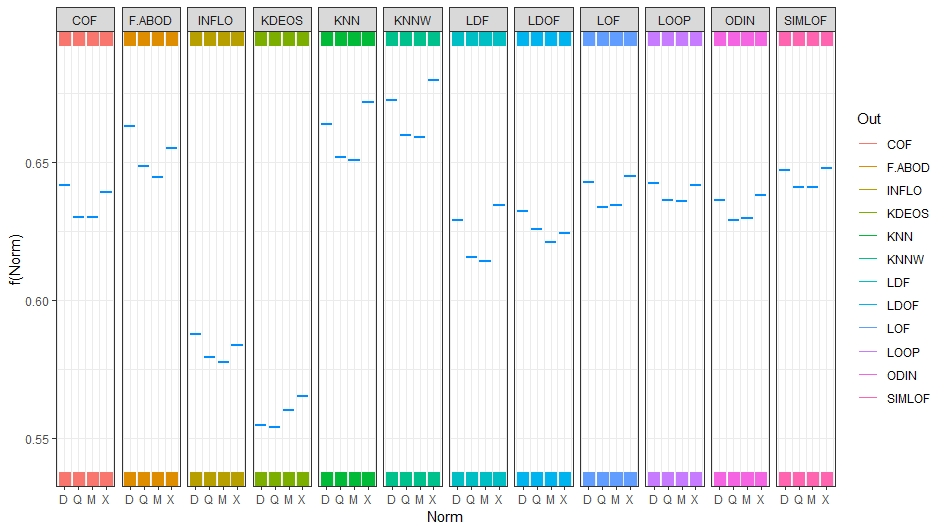
\includegraphics[scale=0.4]{fit3_Norm_Effect_By_Out.jpeg}
    \end{figure}
    \end{frame}	
 		
 	\begin{frame}[noframenumbering,plain]{More results \ldots}
 	\begin{itemize}
 	    \item About 50\% of datasets prefer Median-IQR  to Min-Max
 	    \item Some datasets are more sensitive to normalization than others
 	    \item Some outlier methods are more sensitive to normalization than others
 	    \item Use meta-features to predict sensitivity to normalization with 75\% accuracy
 	    \item A bit more difficult to predict which normalization method to use
 	\end{itemize}
 	    
 	\end{frame}	
 	\begin{frame}[noframenumbering,plain]{Takeaway}
 	    \begin{itemize}
 			\item 	Normalization is an important ``parameter'' of outlier detection techniques.
 			\vspace{0.5cm}
 			\item  Fixing the normalization method has its consequences.
 			\vspace{0.5cm}
 			\item  Find the best normalization that suits the dataset.
 		\end{itemize}
 		 
 	\end{frame}
 		
 	\begin{frame}[noframenumbering,plain,label=figsnorm]
		\begin{figure}[b]
		\centering
		\tikzset{
			head/.style = {fill = none, label = center:\textsf{H}},
			tail/.style = {fill = none, label = center:\textsf{T}}}
		\scalebox{0.65}{\begin{tikzpicture}[
			scale = 1.5, transform shape, thick,
			every node/.style = {draw, circle, minimum size = 10mm},
			grow = down,  % alignment of characters
			level 1/.style = {sibling distance=3cm},
			level 2/.style = {sibling distance=4cm},
			level 3/.style = {sibling distance=2cm},
			level distance = 2.25cm]
			\node[shape = rectangle,
			minimum width = 6cm, minimum height = 1.5cm, font = \sffamily, rounded corners, fill={rgb:red,0;green,176;blue,80}] {Algorithm Selection};
			

			% Labels
		\end{tikzpicture}}
	\end{figure}
	
	\end{frame}
 		
 \begin{frame}[noframenumbering,plain]{Research Question 1}
 	\begin{figure}[!t]
 	\centering
 	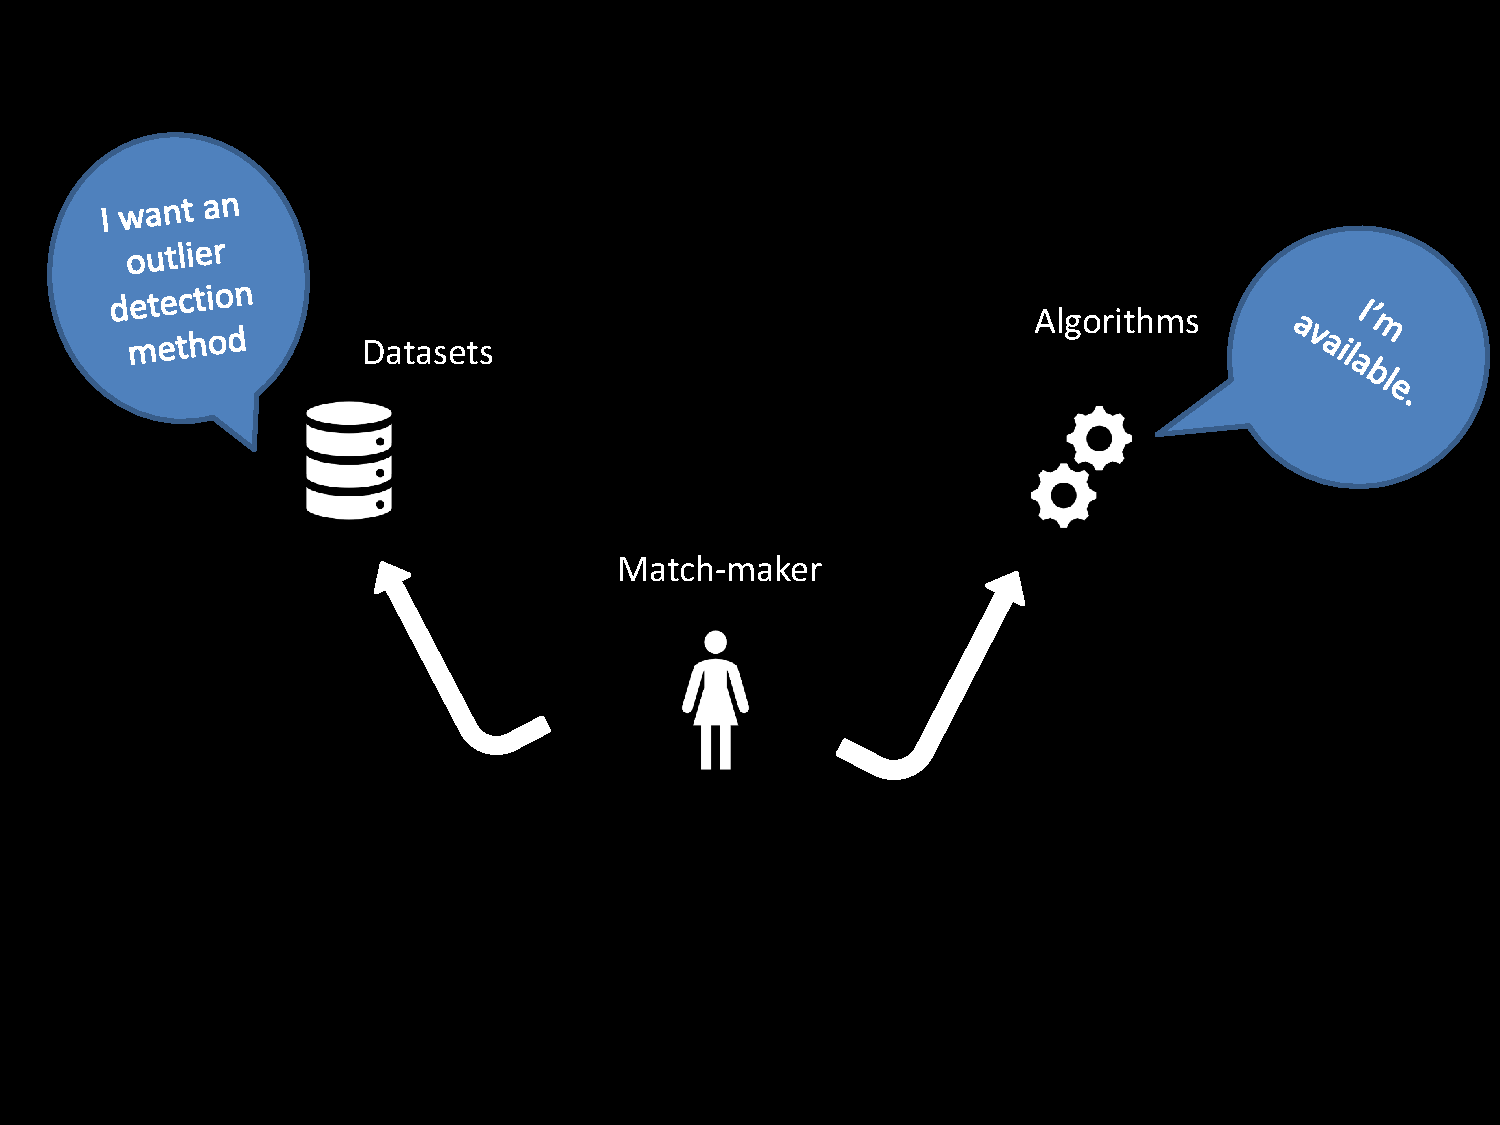
\includegraphics[clip=true, height=6.45cm]{match_maker.pdf}%width=0.40\textwidth, clip
   	\end{figure}
 	\end{frame}	
 	
\begin{frame}[noframenumbering,plain]{Predict outlier method using meta-features}
    \begin{table}[!t]
	\centering
	\footnotesize
	\begin{tabular}{p{3.5cm}p{3cm}p{3cm}}
		\toprule
		Outlier detection method & Default accuracy(\%)  & Prediction accuracy(\%)       \\
		\midrule
		COF                      & 75.58      & 83.48                   \\
		FAST ABOD                & 67.77      & 86.07                    \\
		INFLO                    & 83.22      & 89.29                    \\
		KDEOS                    & 90.96      & 92.81                    \\
		KNN                      & 68.16      & 86.56                    \\
		KNNW                     & 67.13      & 86.13                     \\
		LDF                      & 75.65      & 85.28                    \\
		LDOF                     & 80.08      & 87.36                   \\
		LOF                      & 74.63      & 84.07                    \\
		LOOP                     & 77.19      & 85.88                     \\
		ODIN                     & 79.09      & 87.00                    \\
		SIMLOF                   & 75.85      & 85.21                    \\
		\bottomrule
	\end{tabular}
	\label{table:predOutPerf}
\end{table}
\end{frame}

\begin{frame}[noframenumbering,plain]{Takeaway}
\begin{itemize}
    \item No outlier method is superior to all other methods \\ \vspace{0.5cm}
    \item Need to find the suitable method for a given problem \\ \vspace{0.5cm}
    \item We use meta-features to do the mapping
\end{itemize}
    
\end{frame}

    \begin{frame}[noframenumbering,plain]
    \begin{figure}[b]
		\centering
		\tikzset{
			head/.style = {fill = none, label = center:\textsf{H}},
			tail/.style = {fill = none, label = center:\textsf{T}}}
		\scalebox{0.65}{
		\begin{tikzpicture}[
			scale = 1.5, transform shape, thick,
			every node/.style = {draw, circle, minimum size = 10mm},
			grow = down,  % alignment of characters
			level 1/.style = {sibling distance=3cm},
			level 2/.style = {sibling distance=4cm},
			level 3/.style = {sibling distance=2cm},
			level distance = 2.25cm
			]
			\node[shape = rectangle,
			minimum width = 4cm, font = \sffamily, rounded corners, fill={rgb:red,0;green,176;blue,80}] {Outlier Detection}% fill=black!60!green
			child { node[shape = rectangle, draw, line width = 1pt,
				minimum width = 4cm, xshift=-1.5cm, rounded corners, fill={rgb:red,0;green,176;blue,80}] (Start){Normalization}
			}
			child { node[shape = rectangle, draw, line width = 1pt,
				minimum width = 4cm, xshift=1.5cm, rounded corners, fill={rgb:red,0;green,176;blue,80}] (Start){Algorithm Selection}
			};
			
			% Filling the root (Start)
			\begin{scope}[on background layer, rotate=30]
			\fill[head] (Start.base) ([xshift = 0mm]Start.east) arc (0:180:5mm)
			-- cycle;
			\fill[tail] (Start.base) ([xshift = 0pt]Start.west) arc (180:360:5mm)
			-- cycle;
			\end{scope}
			
			% Labels
		\end{tikzpicture}}
	\end{figure}
 	\end{frame}
 	
 	\begin{frame}[noframenumbering,plain]{Thank you!}
 	\centering
 	\begin{itemize}
 		\item R package \textit{outselect} at https://github.com/sevvandi/outselect
 		\vspace{1cm}
 		\item  Pre-print on research gate: On normalization and algorithm selection for unsupervised outlier detection 
 	\end{itemize}
 
 		
 	\end{frame}
  	\end{darkframes}
\end{document}
